\documentclass[12pt]{article}
\usepackage{setspace}
\setlength{\parindent}{4em}
\usepackage{fancyvrb}
\usepackage{graphicx}
\usepackage{geometry}
\renewcommand\thesection{\arabic{section}}
\renewcommand\thesubsection{\thesection.\arabic{subsection}}
\geometry{letterpaper, portrait, margin=1in}

%%%Title Page%%%
\title{\vspace{3cm}Lab 03\bigbreak Designing the Toy Processor Datapath}
\author{
{\normalsize
\begin{tabular}{l r r}
 & \textbf{Ryan Cruz} & \textbf{Zachary Davis}\\
\textbf{Category} & ryan.cruz25@uga.edu & zachdav@uga.edu\\
\hline
Pre-lab 						  & 50 & 50\\
In-lab Module \& Testbench Design & 50 & 50\\
In-lab Testbench Sim. \& Analysis & 50 & 50\\
In-lab FPGA Synthesis \& Analysis & 50 & 50\\
Lab Report Writing 				  & 50 & 50\\
\end{tabular}
}}
%%%%%%%%%%%%%%%%%

\begin{document}
\maketitle
\newpage
\setstretch{2.5} % for custom spacing
\tableofcontents
\setstretch{1} % for custom spacing
\newpage

\section{Lab Purpose} \vspace{-.7cm} \line(1,0){470}
	\paragraph{} The purpose of this lab is to create/design the necessary components for our Toy Processor Datapath. This includes building an 8-bit register for Instruction and Data Registers, a counter for the program counter, and a design for putting it all together. 				
\section{Implementation Details} \vspace{-.7cm} \line(1,0){470}
		\subsection{Part 1}
		First, we built an 8-bit register that will be used for the instruction and data registers. 
		\begin{center}
			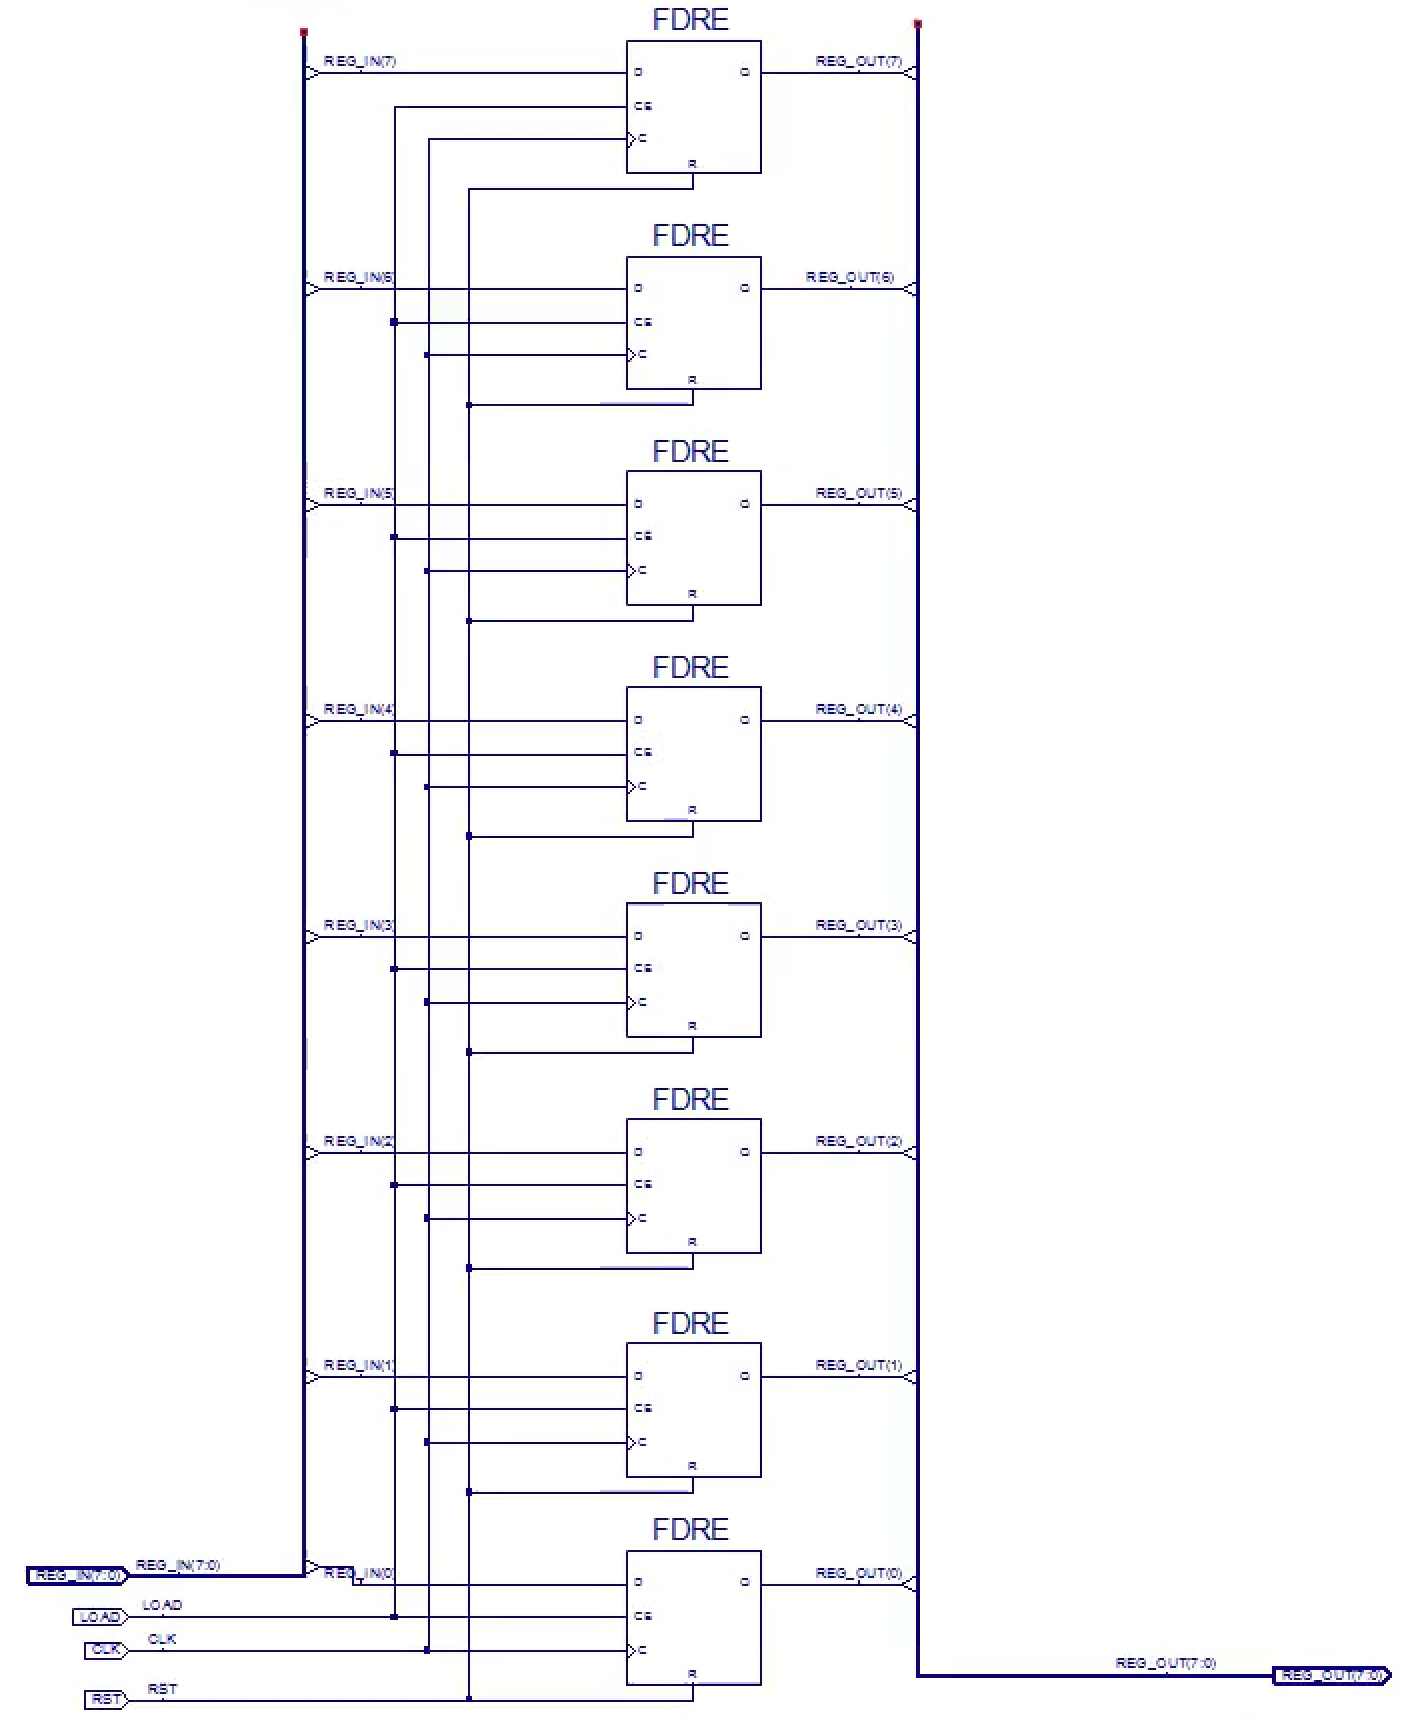
\includegraphics[scale=.5]{reg_sch.png}
		\end{center}
	
		\begin{Verbatim}[frame=single, fontsize= \small]
`timescale 1ns/1ps
	
	module reg_tbw_tb_0;
		reg CLK = 1'b0;
		reg LOAD = 1'b0;
		reg [7:0] REG_IN = 8'b00000000; 
		reg RST = 1'b0;
		
		wire [7:0] REG_OUT;
	
		parameter PERIOD = 200; 
		parameter real DUTY_CYCLE = 0.5; 
		parameter OFFSET = 100;
		
		initial // Clock process for CLK 
			begin
				#OFFSET; 
				forever 
					begin
						CLK = 1'b0; 
						#(PERIOD-(PERIOD*DUTY_CYCLE)) 
							CLK = 1'b1; 
						#(PERIOD*DUTY_CYCLE);
					end 
			end
	
		reg_sch UUT (
			.CLK(CLK), 
			.LOAD(LOAD), 
			.REG_IN(REG_IN), 
			.RST(RST), 
			.REG_OUT(REG_OUT));
	
		initial 
			begin
	
				// ------------- Current Time: 185ns 
				#185;
				LOAD = 1'b1;
	
				// -------------------------------------
				// ------------- Current Time: 385ns 
				#200;
				REG_IN = 8'b00000001;
	
				// -------------------------------------
				// ------------- Current Time: 585ns
				#200;
				LOAD = 1'b0;
				REG_IN = 8'b00000010;
		
				// -------------------------------------
				// ------------- Current Time: 785ns 
				#200;
				REG_IN = 8'b00000011;
	
				// -------------------------------------
				// ------------- Current Time: 985ns 
				#200;
				LOAD = 1'b1;
				RST = 1'b1;
				REG_IN = 8'b00000100;
	
				// -------------------------------------
				// ------------- Current Time: 1185ns 
				#200;
				RST = 1'b0;
				REG_IN = 8'b00000101;
	
				// -------------------------------------
				// ------------- Current Time: 1385ns 
				#200;
				REG_IN = 8'b00000110;
	
				// -------------------------------------
				// ------------- Current Time: 1585ns 
				#200;
				REG_IN = 8'b00000111;
			end 
	endmodule			
		\end{Verbatim}

	\newpage
	\subsection{Part 2}
		
		\begin{center}
			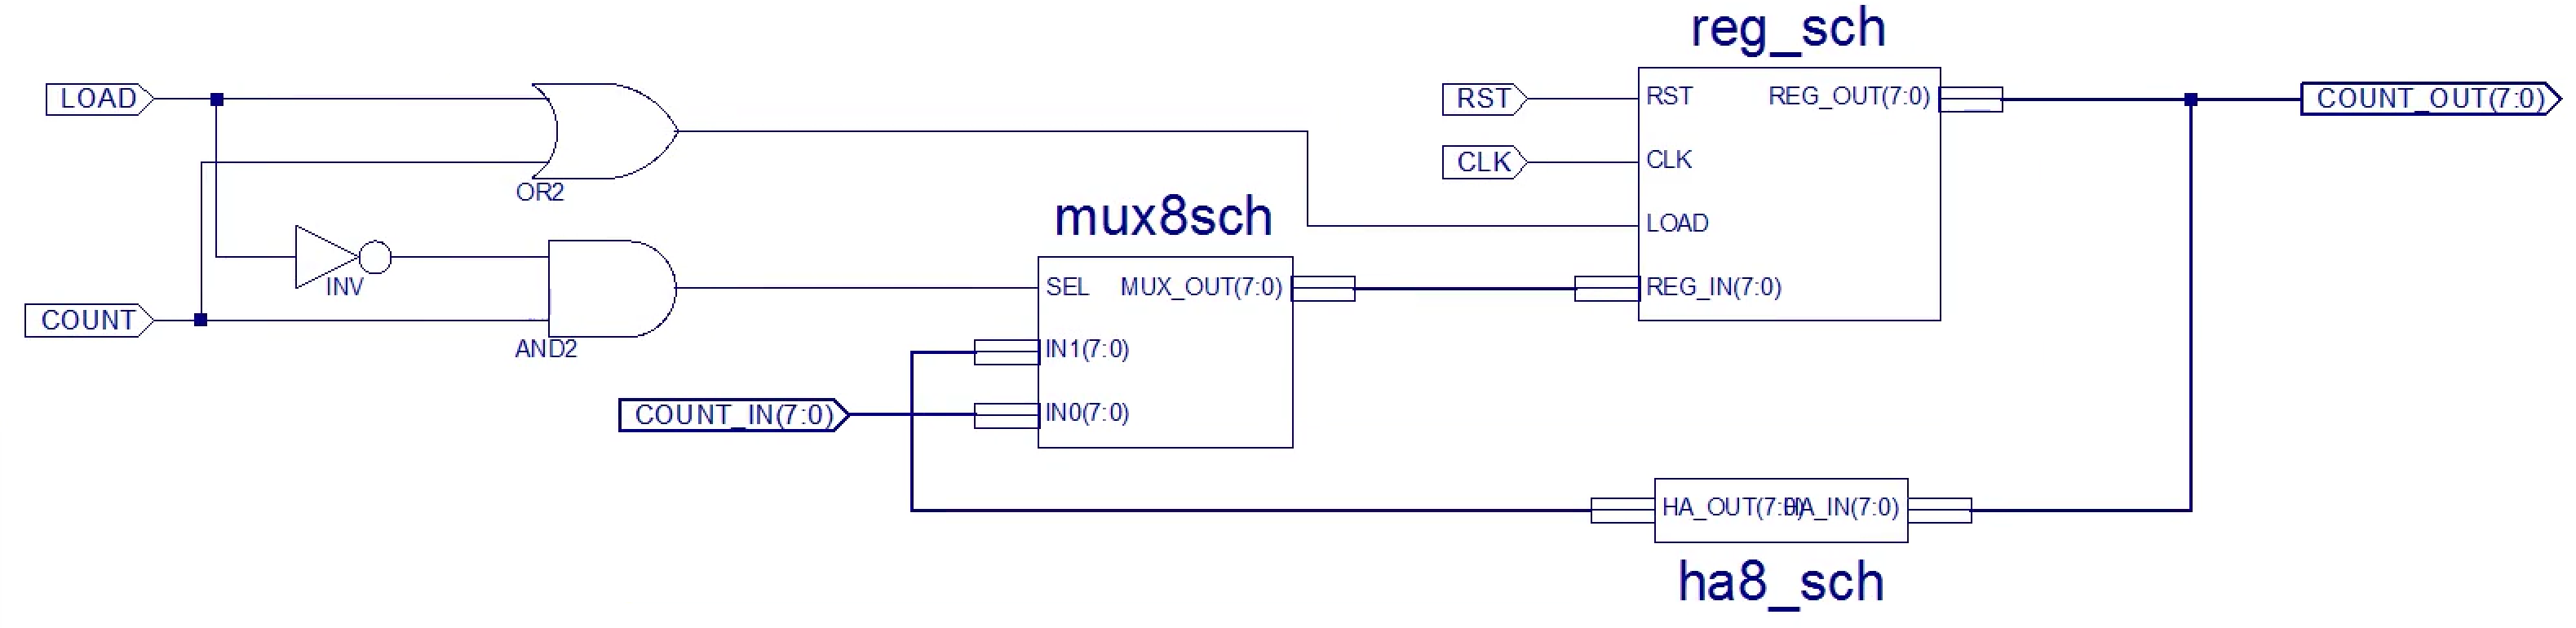
\includegraphics[scale=.31]{counter_sch.png}
		\end{center}

		\begin{Verbatim}[frame=single, fontsize=\small]
`timescale 1ns/1ps

	module counter_tbw_tb_0;
		reg CLK = 1'b0;
		reg COUNT = 1'b0;
		reg [7:0] COUNT_IN = 8'b00000000; 
		reg LOAD = 1'b0;
		reg RST = 1'b0;
		
		wire [7:0] COUNT_OUT;
		
		parameter PERIOD = 200; 
		parameter real DUTY_CYCLE = 0.5; 
		parameter OFFSET = 100;

		initial // Clock process for CLK 
			begin
				#OFFSET; 
				forever 
					begin
						CLK = 1'b0; 
						#(PERIOD-(PERIOD*DUTY_CYCLE)) 
							CLK = 1'b1; 
						#(PERIOD*DUTY_CYCLE);
					end 
			end
		
		counter_sch UUT ( 
			.CLK(CLK), 
			.COUNT(COUNT), 
			.COUNT_IN(COUNT_IN),
			.LOAD(LOAD),
			.RST(RST), 
			.COUNT_OUT(COUNT_OUT));
			
		initial 
			begin
				// ------------- Current Time: 185ns 
				#185;
				RST = 1'b1;
				
				// -------------------------------------
				// ------------- Current Time: 585ns 
				#400;
				COUNT_IN = 8'b00000001;
				
				// -------------------------------------
				// ------------- Current Time: 785ns 
				#200;
				RST = 1'b0;
				COUNT_IN = 8'b00000010;
				
				// -------------------------------------
				// ------------- Current Time: 985ns 
				#200;
				COUNT_IN = 8'b00000011;
				
				// -------------------------------------
				// ------------- Current Time: 1185ns 
				#200;
				LOAD = 1'b1;
				COUNT_IN = 8'b00000100;
				
				// -------------------------------------
				// ------------- Current Time: 1385ns 
				#200;
				COUNT = 1'b1;
				COUNT_IN = 8'b00000101;
				
				// -------------------------------------
				// ------------- Current Time: 1585ns 
				#200;
				COUNT = 1'b0;
				LOAD = 1'b0;
				COUNT_IN = 8'b00000110;
				
				// -------------------------------------
				// ------------- Current Time: 1785ns 
				#200;
				COUNT_IN = 8'b00000111;
				
				// -------------------------------------
				// ------------- Current Time: 1985ns 
				#200;
				COUNT = 1'b1;
				COUNT_IN = 8'b00001000;
				
				// -------------------------------------
				// ------------- Current Time: 2185ns 
				#200;
				COUNT_IN = 8'b00001001;
				
				// -------------------------------------
				// ------------- Current Time: 2385ns 
				#200;
				COUNT = 1'b0;
				COUNT_IN = 8'b00001010;
				
				// -------------------------------------
				// ------------- Current Time: 2585ns 
				#200;
				COUNT_IN = 8'b00001011;
				
				// -------------------------------------
				// ------------- Current Time: 2785ns 
				#200;
				COUNT_IN = 8'b00001100;
				
				// -------------------------------------
				// ------------- Current Time: 2985ns 
				#200;
				COUNT_IN = 8'b00001101;
			end 
	endmodule

			
		\end{Verbatim}
\newpage
	\subsection{Part 3}
		Now we can combine the previous parts into a working 4-bit ALU. In essence, we stack the Logic Extender and the Arithmetic Extender onto the Full Adder
		\begin{center}
			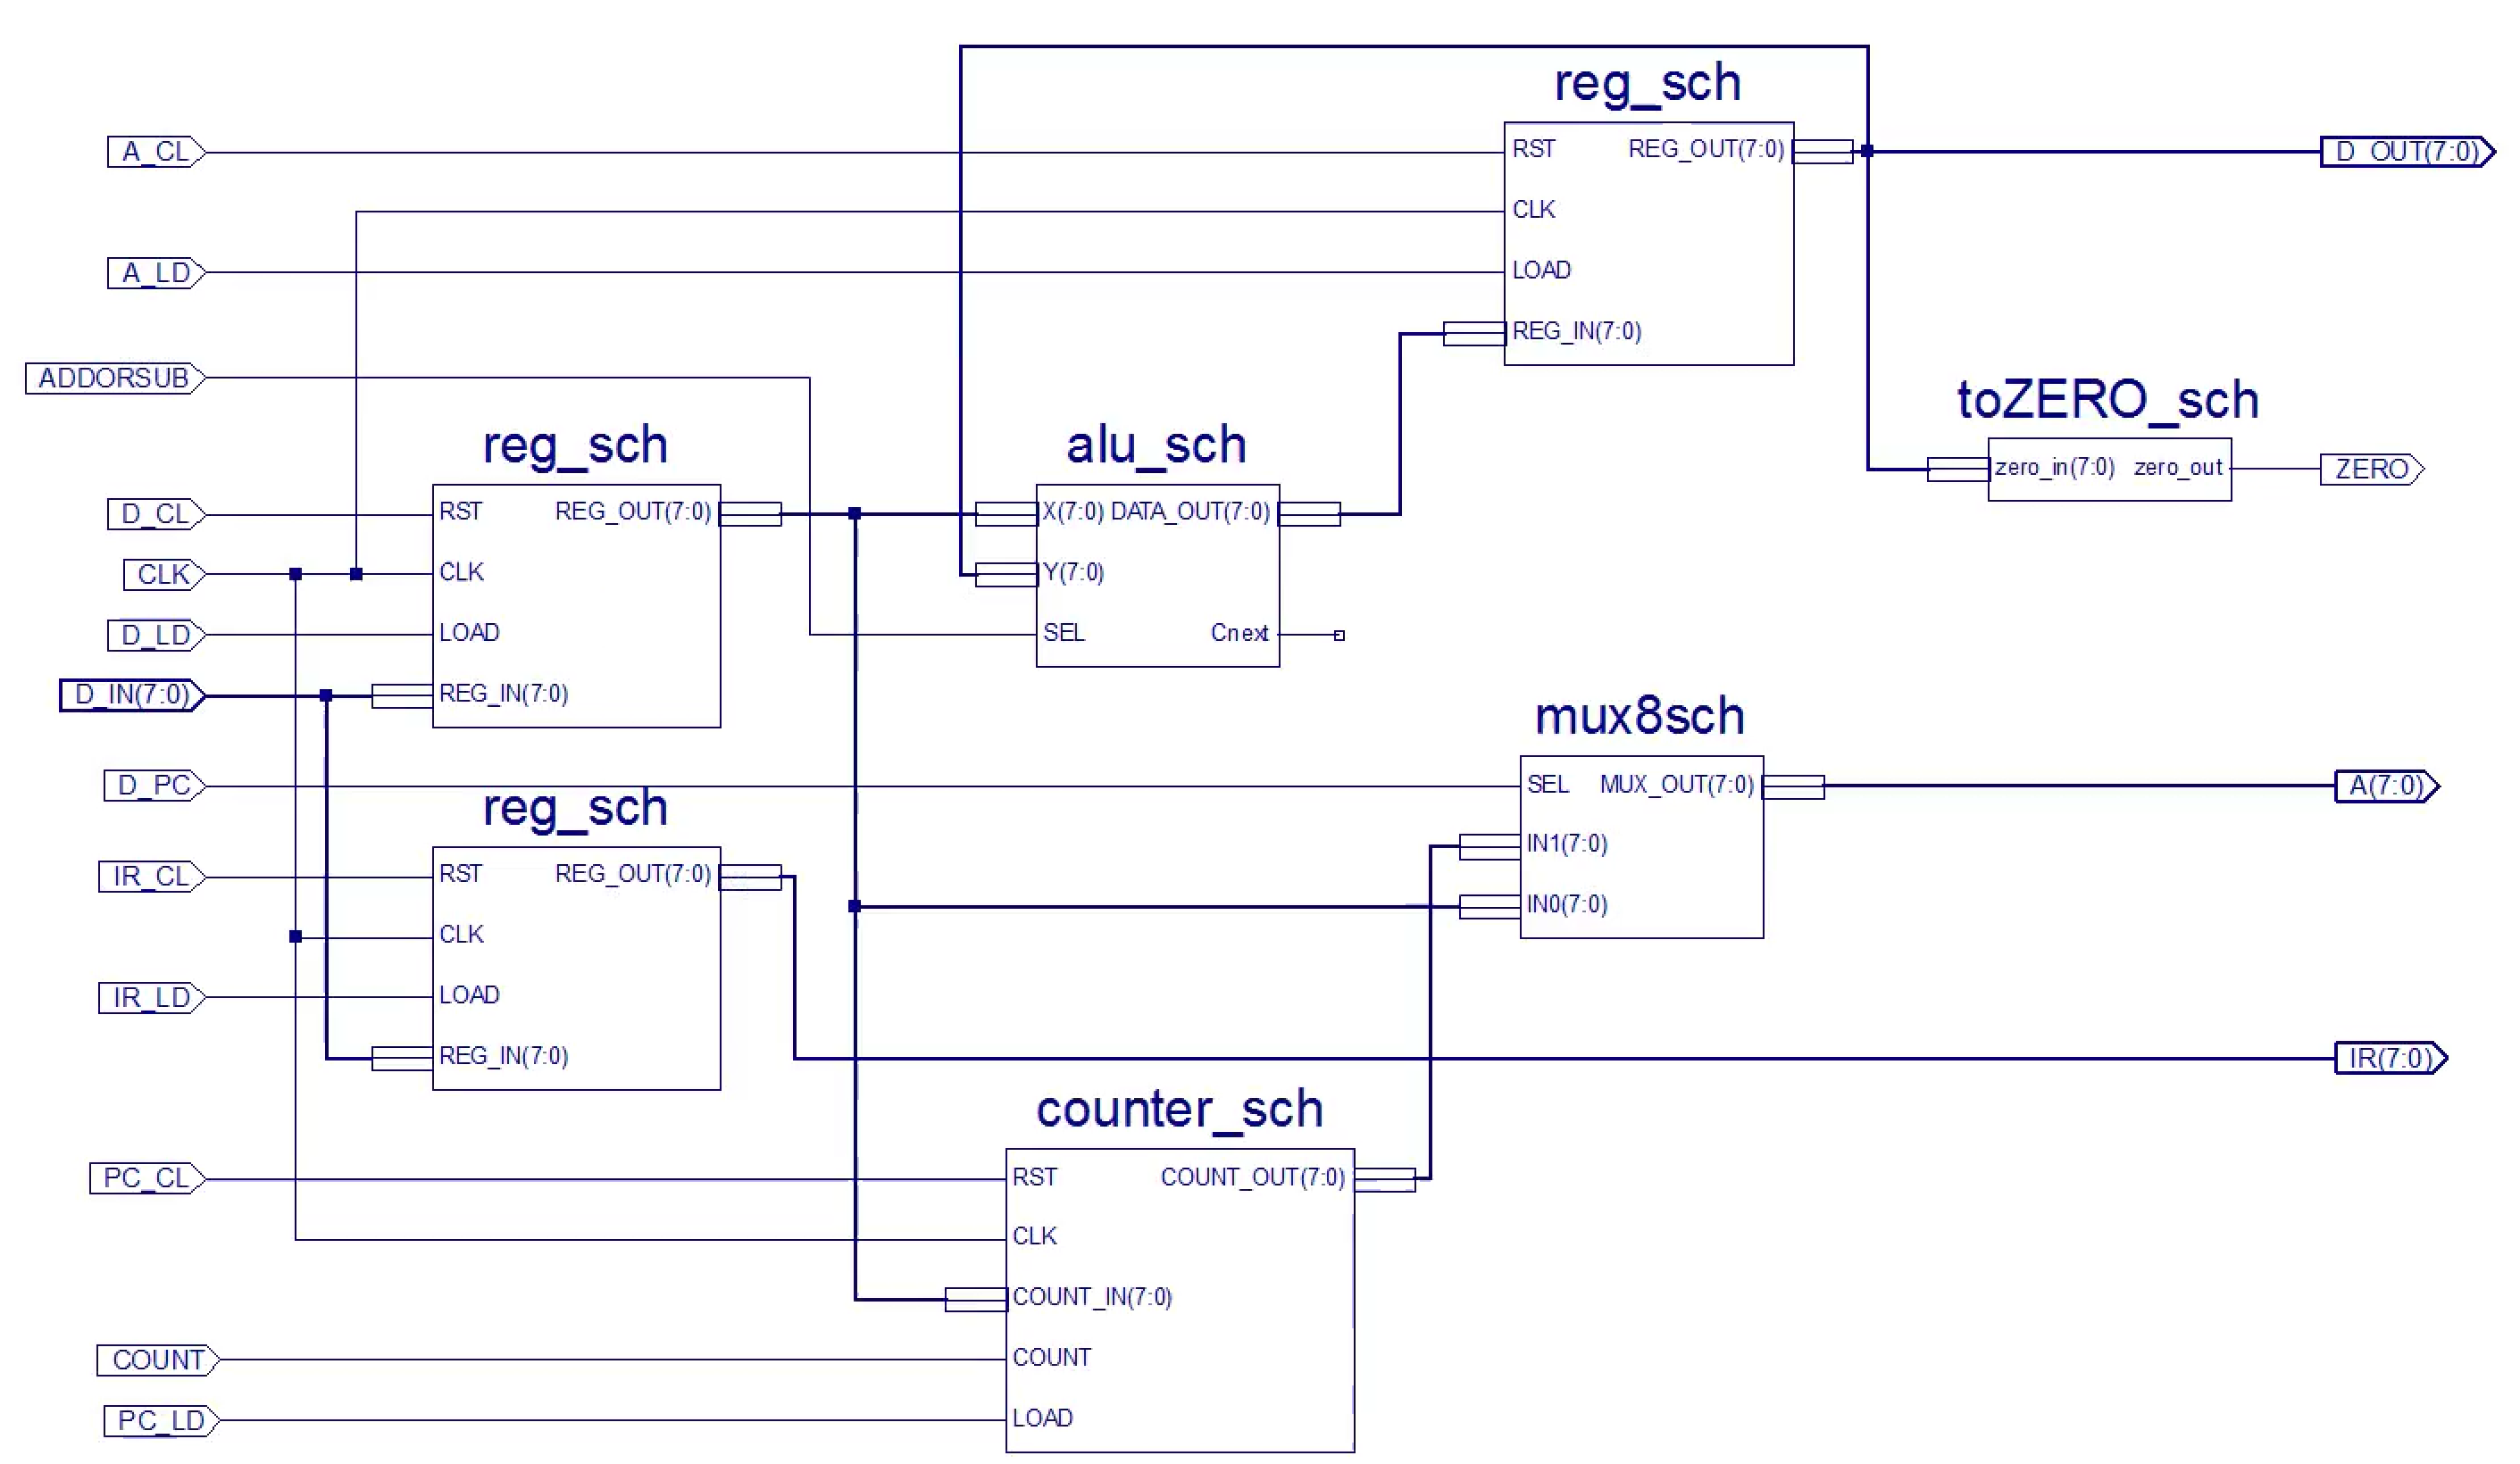
\includegraphics[scale=.3]{datapath.png}
		\end{center}
\newpage
		\begin{Verbatim}[frame=single, fontsize=\small]

			
		\end{Verbatim}
			
\section{Experimental Results}\vspace{-.7cm} \line(1,0){470}

%\begin{figure}[h]
%    \centering
%	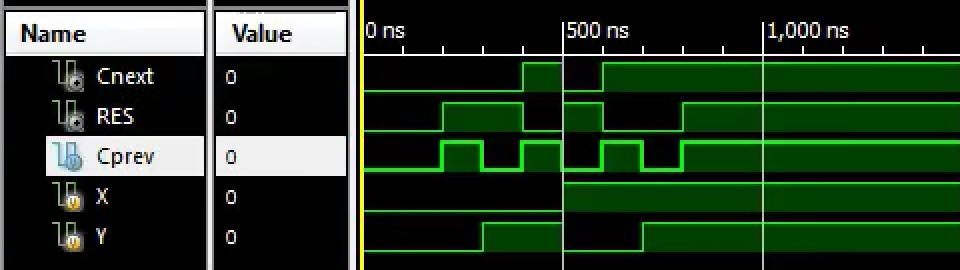
\includegraphics[scale=.7]{fa_tb_wave.png}
%	\caption{Waveform for the full adder schematic test bench. All test cases present for each value of X, Y, and Cprev, showing successful binary addition and carrying.}
%\end{figure}
%
%%\begin{figure}
%%	\includegraphics[scale=.7]{alu_tb_wave.png}
%%\end{figure}
%
%\begin{figure}[h]
%    \centering
%	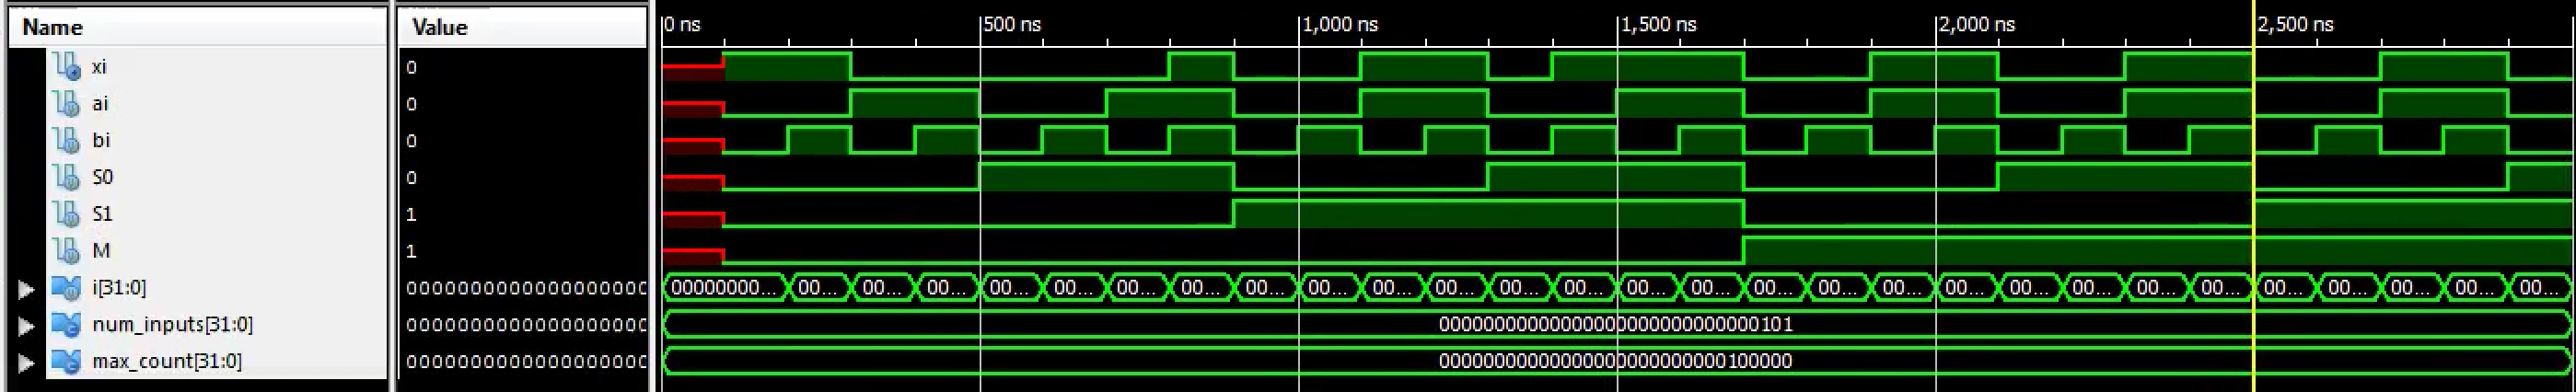
\includegraphics[scale=.33]{logic_ext_tb_wave}
%	\caption{Waveform for the logic extender schematic test bench. All test cases match that of the table given, successfully performing all required logic operations}
%\end{figure}
%
%\begin{figure}[h]
%    \centering
%	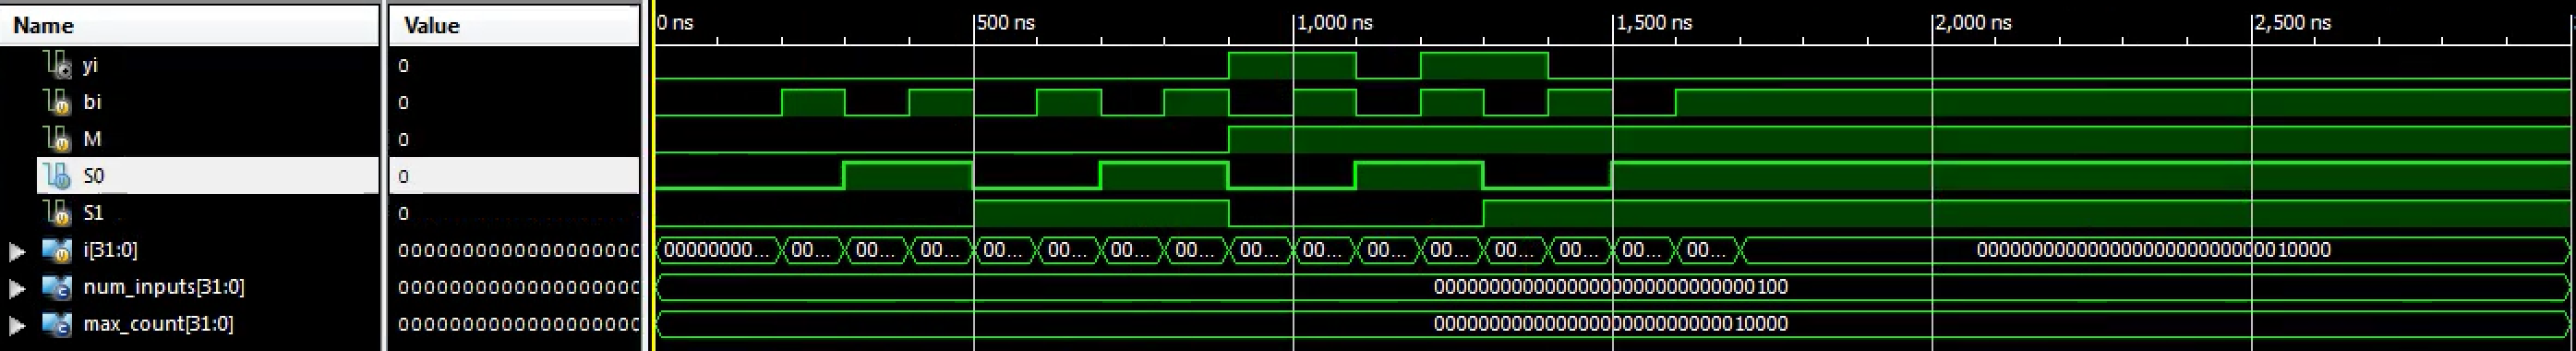
\includegraphics[scale=.33]{arith_ext_tb_wave.png}
%	\caption{Waveform for the arithmetic extender schematic test bench. All test cases match that of the table given, successfully performing all required arithmetic operations}
%\end{figure}
%
%\begin{figure}[h]
%    \centering
%	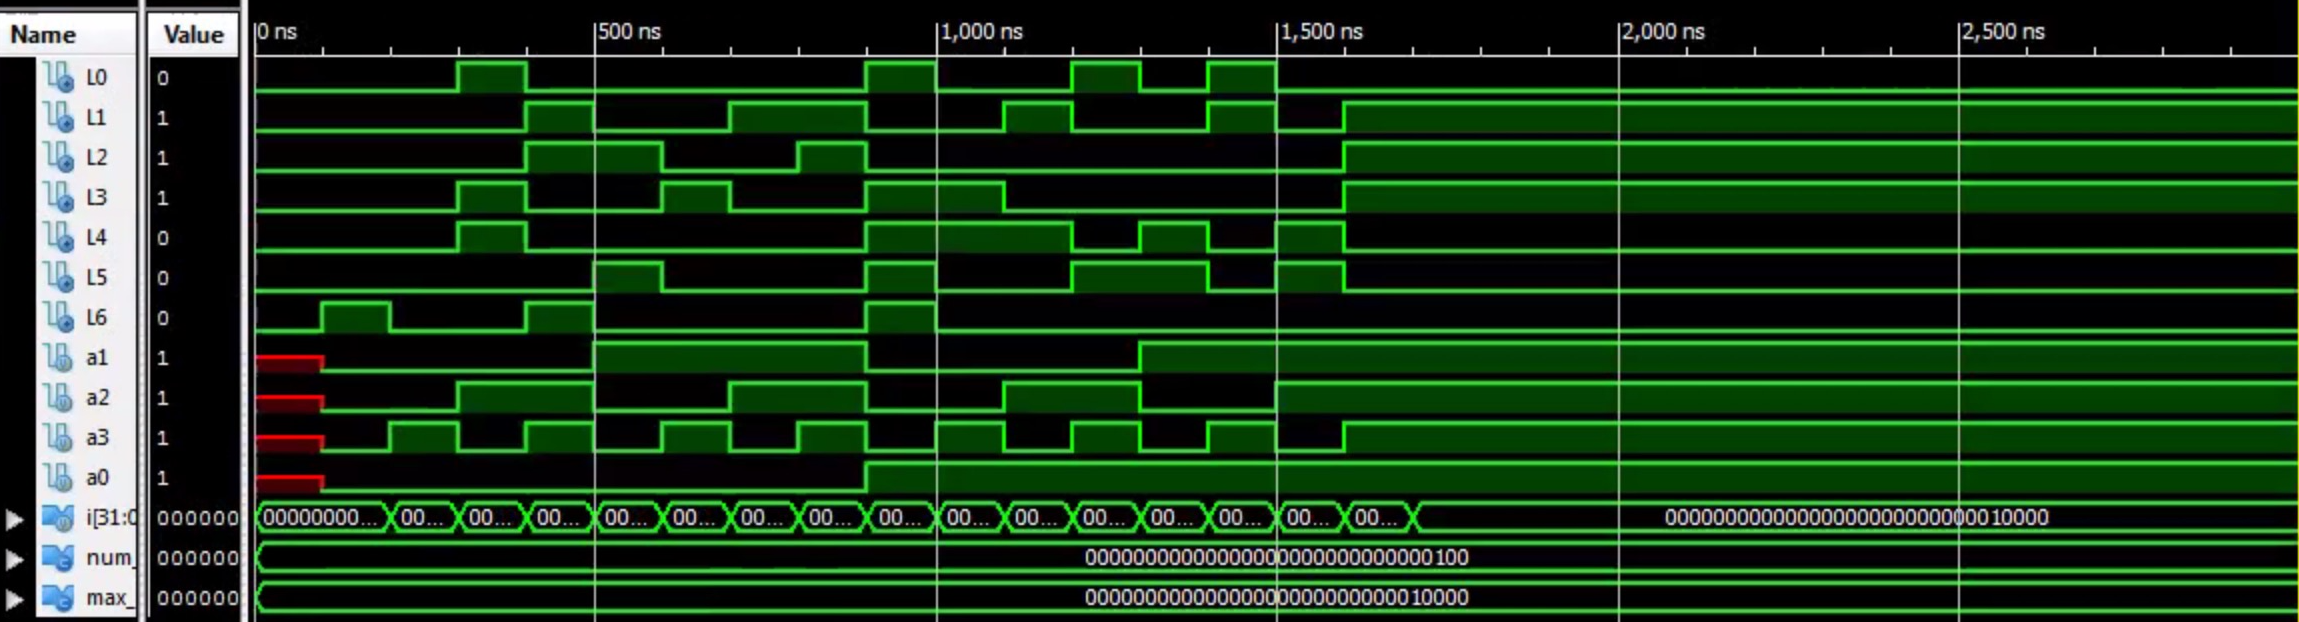
\includegraphics[scale=.2]{seven_segment_tb_wave.png}
%	\caption{Waveform for the seven segment display driver, showing all possible combinations for the 4-bit binary input, and corresponding outputs.}
%\end{figure}
%
%\begin{figure}[ht]
%    \centering
%	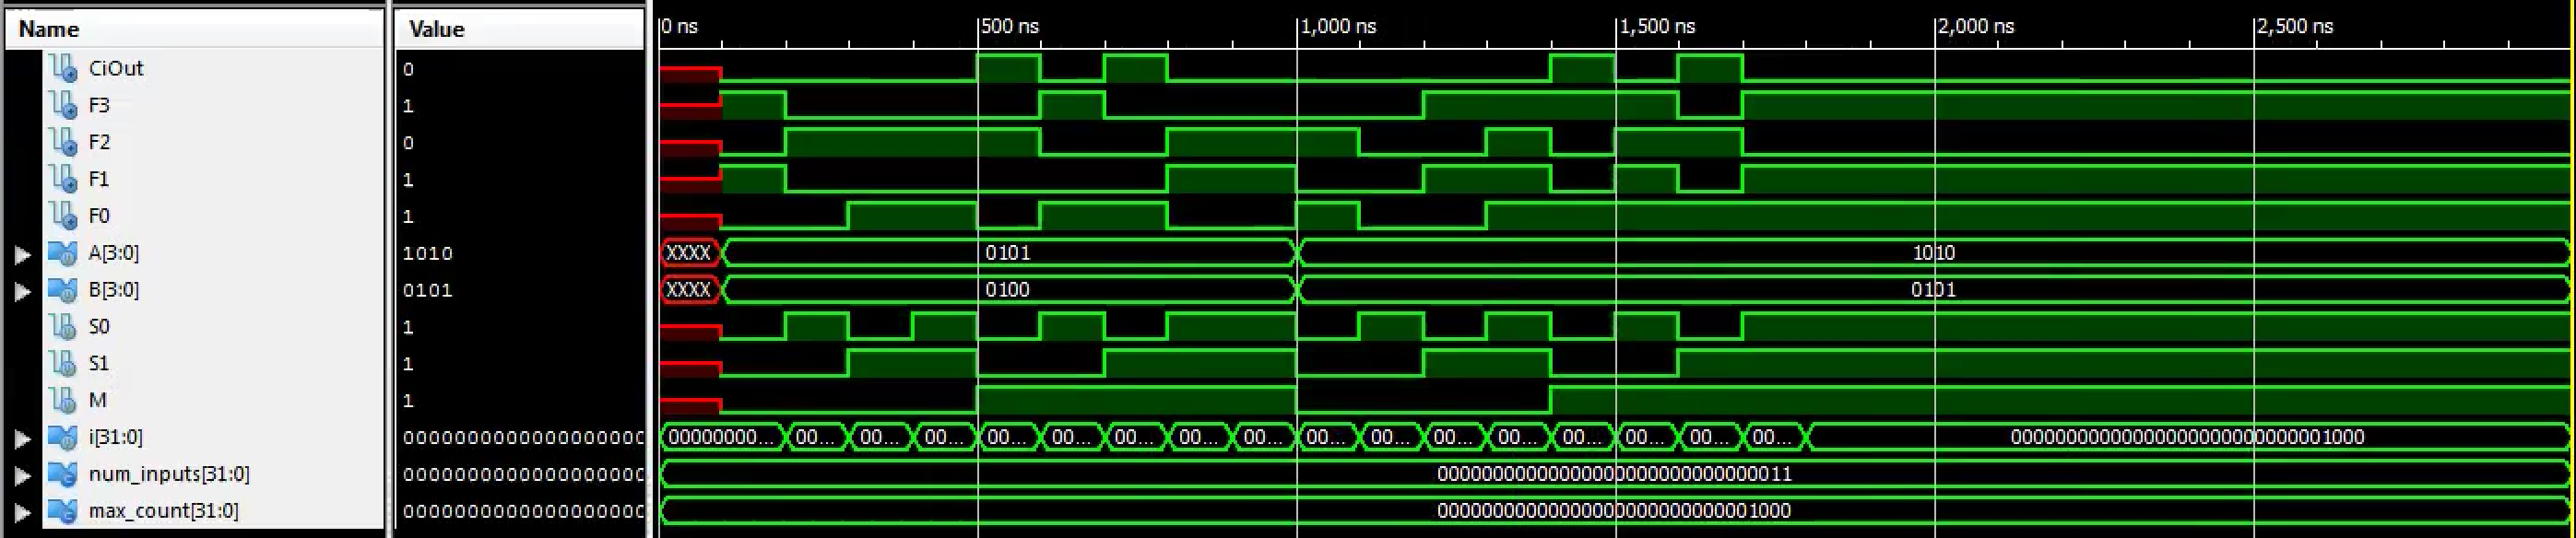
\includegraphics[scale=.33]{alu4bit_tb_wave.png}
%	\caption{Waveform for the 4-bit ALU, testing again each possible input combination of S0, S1, and M.}
%\end{figure}

	\newpage
\section{Significance} \vspace{-.7cm} \line(1,0){470}
	\paragraph{}
		This lab was the first comprehensive use of the Xilinx GUI schematic creator, and using it to create several modules that would eventually create a full project, and eventually exist on the board. While this did feel like a full, independent project of its own, in reality it is just the first piece of a much bigger puzzle that is a usable CPU. With the knowledge gained in this lab, piecing the parts together makes much more sense now. 

 \section{Comments/Suggestions}\vspace{-.7cm} \line(1,0){470}
 	\paragraph{}
		Everything was rather straightforward, although it was relatively quite a bit of work. In the future, it may be best to assign a portion of the lab as prelab, so that it could be more spread out.
		
\end{document}


